\documentclass[main.tex]{subfiles}

\begin{document}

	\begingroup

	\renewcommand{\cleardoublepage}{}

	\renewcommand{\clearpage}{}

	\chapter{Architecture Overview}
		In order to cope with the challenges we were facing as mentioned in the introduction they have been summarized into five groups:

		\begin{itemize}
			\item Navigation: Movement and localization
			\item Perception: Recognition of objects and classification
			\item Knowledge: Storage and providing access to information about the world state and object positions within the world
			\item Manipulation: Interaction with the world and objects within the world
			\item Planning: Decision making, execution and error handling
		\end{itemize}


		\chapterauthor{}
		
		\section{Diagram}
		
		\begin{figure}[h]
			\centering
			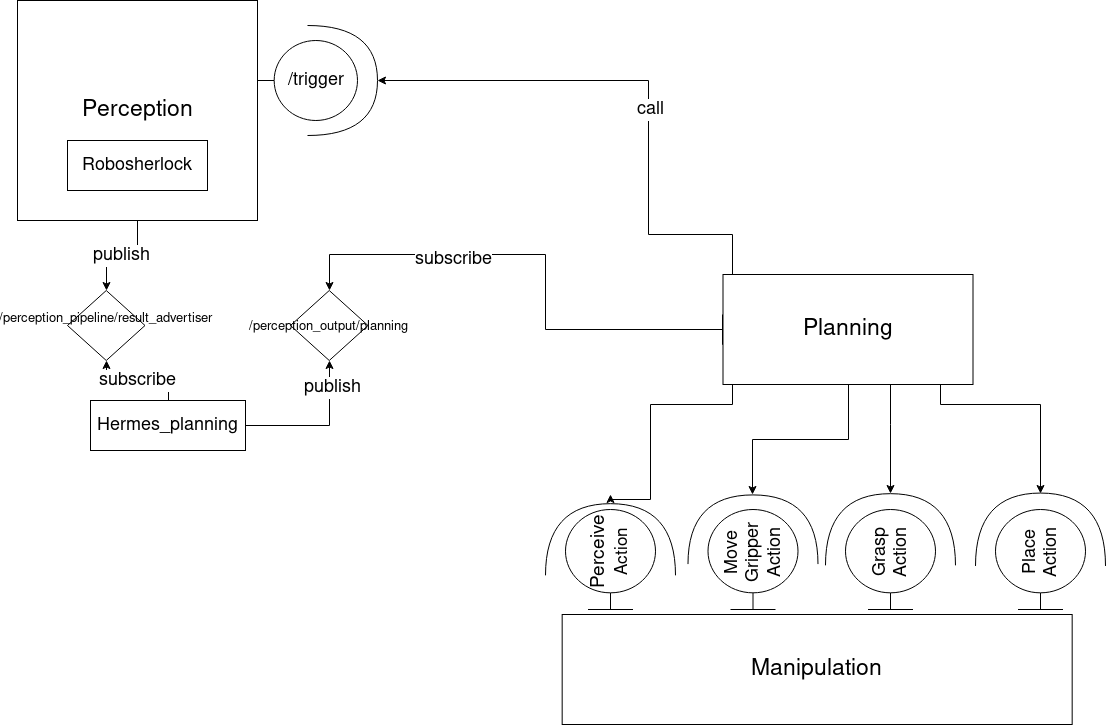
\includegraphics[width=0.85\textwidth]{pictures/diagramms/architecture.png}
			\caption{Architecture overview}
			\label{architecture}
		\end{figure}
		
		\section{Description}
			As seen in the diagramm \(\ref{architecture}\), the component which each group was responsible for are visualized. The perception component consists mainly off the SuturoProcessManager module which wraps the robosherlock pipeline (HIER PERCEPTION BITTE BESSER ERLÄUTERN). The robosherlock pipeline then handles the classification and annotation blah blah blah usw. The Knowledge component consists of the knowledge base which is basically a wrapped information storage (database) of the HSR it handles position data aswell as some logic for goal position determination. The Manipulation component is responsible for gripper movement, head and body movement as well as grasp and place operations. For this Manipulation is using Giskard. The Navigation component is only used for moving the HSR and for collision avoidance during movement. The Planning component uses cram which is a 
			\begin{itemize}
				\item{\textbf{Cram}} \\
					 Cram is a software toolbox for the design, the implementation, and the deployment of cognition-enabled autonomous robots
				\item{\textbf{Giskard}} \\
					giskard is a  framework for constraint based motion planning and execution.
				\item{\textbf{Julius}} \\
					Julius is a continuous speech recognition software. It is capable of recognizing spoken sentence as-live. Julius' main strength is the fact, that it works on dictionaries. Dictionaries are a spimple way for developers to adapte Julius to only recognize domain-specific sentences. Julius is not specifically created for ROS, but Toyota created a wrapper to allow the output of Julius to be published in ROS.
				\item{\textbf{KnowRob}} \\
				    KnowRob is a framework created to combine different knowledge sources (such as knowledge about and provided by the robot, common sense, research etc.) and provide some reasoning methods to work with them. 
				\item{\textbf{Robosherlock}} \\
					RoboSherlock is a common framework for cognitive perception, based on the principle of unstructured information management (UIM).
				\item{\textbf{Caffee}} \\
					Caffe is a deep learning framework made with expression, speed, and modularity in mind. It is developed by Berkeley AI Research (BAIR) and by community contributors.

			\end{itemize}
		
			The planning component as seen in \ref{architecture} is basically the connection piece and main executor for the low level robot operations performed by the other components. It basically consists of three packages although the most top level package(execute) was split for the both tasks, the other packages common-functions and low-level-interfacing are explained in following chapters. The planning component initializes connections to the action servers of th other components and sends requests to perform robot actions or as for the access the world representation and knowledge of the robot.
	  		 

	\endgroup

\end{document}
